\documentclass[aspectratio=169]{beamer}
\usetheme[progressbar=frametitle, numbering=none]{metropolis}
 % Modern, minimal theme
\setbeamertemplate{footline}{
  \leavevmode%
  \hbox{%
  \begin{beamercolorbox}[wd=.95\paperwidth,ht=2.5ex,dp=1ex,leftskip=1em]{author in head/foot}%
    \usebeamerfont{author in head/foot}\insertshortauthor\hspace{1em}-- \insertshortinstitute
  \end{beamercolorbox}%
  \begin{beamercolorbox}[wd=.3\paperwidth,ht=2.5ex,dp=1ex,rightskip=1em]{date in head/foot}%
    \usebeamerfont{date in head/foot}\insertframenumber{} / \inserttotalframenumber
  \end{beamercolorbox}}%

}

\usepackage{graphicx}   % Images
\usepackage{minted}
\usepackage{booktabs}   % Tables
\usepackage{amsmath}    % Math support
\usepackage{caption}
\captionsetup[figure]{labelfont={scriptsize}, textfont={scriptsize}}
% Code blocks (use -shell-escape to compile)
\usepackage{tikz}       % Diagrams (optional)

% Metadata
\title{I/O Performance trade-offs among RNTuple’s persistent layouts for DUNE Data Products}
\subtitle{Mentored by Philippe Canal}
\author{S M Shovan, \textit{FCSI Summer Intern'25}}

\institute{Fermi National Accelerator Laboratory}
\date{\today}

\begin{document}

% Title Slide
\maketitle


% Outline
\begin{frame}{Outline}
\tableofcontents
\end{frame}

\section{Introduction}

\begin{frame}{Introduction}
  \begin{itemize}
    \item The Deep Underground Neutrino Experiment (DUNE) is projected to record roughly 30~PB of liquid‑argon TPC data per year\,[1]—far beyond the scale of previous neutrino experiments.
    \item DUNE is developing a new framework: \textbf{Phlex} stands for \textbf{P}arallel, \textbf{h}ierarchical, and \textbf{l}ayered \textbf{ex}ecution of data-processing algorithms.
    \item ROOT’s new \texttt{RNTuple} storage container is a candidate for the long‑term DUNE data model, promising faster compression, cluster‑aware reads, and thread‑safe writes.
    \item This study benchmarks alternative RNTuple \emph{persistent layouts} (AOS/SOA, vertical splits, granularity levels) for realistic data products.
    \item Focus data products: \texttt{recob::Hit} (charge deposits) and \texttt{recob::Wire} (ROI‑compressed waveforms).
  \end{itemize}
\end{frame}

\begin{frame}{Motivation} 
  \begin{itemize}
    \item A single DUNE far‑detector module streams about 1.2\,TB/s of raw data before compression\,[2]; naive storage could potentially overwhelm the archival budget.

    \vspace{2em}

    \item Efficient layout choice can cut file size and accelerate cluster reads needed for GPU/CPU reconstruction farms.
  \end{itemize}
\end{frame}

\begin{frame}{Problem Statement}
  \begin{itemize}
    \item Which RNTuple persistent layout minimises read time, write time and on‑disk footprint for DUNE Hit/Wire data products?
    
    \vspace{2em}

    \item How does vertical splitting such as one RNTuple for all data products or one of each data products interact with horizontal granularities (event, spill, element)?

    \vspace{2em}

    \item How does the choice of persistent layout affect the performance of the read and write operations?
  \end{itemize}
\end{frame}

\begin{frame}{Objectives}
  \begin{itemize}
    \item Benchmark seven layout variants on a 1\,M‑event (35\,GB) Phlex dataset (\texttt{recob::Hit}, \texttt{recob::Wire} with ROIs).
    
    \vspace{2em}

    \item Measure: write throughput, cold/warm read latency, compressed file size.

    \vspace{2em}

    \item Quantify trade‑offs of ROI flattening, vertical split depth, and SOA vs. AOS.
  \end{itemize}
\end{frame}

% -------- Section: Persistent Layouts --------
\section{Persistent Layouts}
\begin{frame}{Data Layouts: AOS vs. SOA}
  \begin{columns}
    \column{0.5\textwidth}
    \textbf{Array of Structures (AOS)} \\
    \small Stores complete objects in an array. 
    \vspace{0.5em}
    \fbox{\parbox{0.9\textwidth}{\small
      \texttt{struct Hit \{ }\\
      \hspace*{1.0em} \texttt{long long EventID; }\\
      \hspace*{1.0em} \texttt{unsigned int fChannel; }\\
      \hspace*{1.0em} \texttt{float fPeakTime; }\\
      \texttt{\}; }\\
      \texttt{// Array: [Hit1, Hit2, ...]}
    }}
    \vspace{0.5em}
    \textbf{Example}: Hit, Wire (per-item entries).

    \column{0.5\textwidth}
    \textbf{Structure of Arrays (SOA)} \\
    \small Separate arrays per field.
    \vspace{0.5em}
    \fbox{\parbox{0.9\textwidth}{\small
      \texttt{struct Hits \{ }\\
      \hspace*{1.0em} \texttt{ vector<long long> EventID; }\\
      \hspace*{1.5em} \texttt{vector<unsigned int> fChannel; }\\
      \hspace*{1.5em} \texttt{vector<float> fPeakTime; }\\
      \texttt{\}; }\\
      \texttt{// Columns: EventID[ ], \\ //fChannel[ ], fPeakTime[ ], ...}
    }}
    \vspace{0.5em}
    \textbf{Example}: Hits, Wires (per-event vectors).
  \end{columns}
  \vspace{1em}
\end{frame}



\begin{frame}{Layout Strategies}

  \begin{columns}
    % Left column (30%)
    \column{0.20\textwidth}
    \centering
    \includegraphics<1->[width=\textwidth]{Figures/AOSLayout.pdf}
    \only<1->{\captionof{figure}{\scriptsize AOS Layout}}

    % Right column (70%)
    \column{0.7\textwidth}
    % Top row (appears on slide 2)
    \begin{columns}
      \column{0.33\textwidth}
      \centering
      \includegraphics<2->[height=0.15\textheight]{Figures/Vertical1.pdf}
      \only<2->{\captionof{figure}{\scriptsize 1 RNTuple for all data products}}

      \column{0.33\textwidth}
      \centering
      \includegraphics<2->[height=0.15\textheight]{Figures/Vertical2.pdf}
      \only<2->{\captionof{figure}{\scriptsize 1 RNTuple per data product}}

      \column{0.33\textwidth}
      \centering
      \includegraphics<2->[height=0.15\textheight]{Figures/Vertical3.pdf}
      \only<2->{\captionof{figure}{\scriptsize 1 RNTuple per group }}
    \end{columns}

    \vspace{0.5em}

    % Bottom row (appears on slide 3)
    \begin{columns}
      \column{0.25\textwidth}
      \centering
      \includegraphics<3->[height=0.13\textheight]{Figures/Hori1.pdf}
      \only<3->{\captionof{figure}{\scriptsize 1 fill/row per event}}

      \column{0.25\textwidth}
      \centering
      \includegraphics<3->[height=0.13\textheight]{Figures/Hori2.pdf}
      \only<3->{\captionof{figure}{\scriptsize 1 fill/row per spill}}

      \column{0.25\textwidth}
      \centering
      \includegraphics<3->[height=0.13\textheight]{Figures/Hori3.pdf}
      \only<3->{\captionof{figure}{\scriptsize 1 fill/row per top object}}

      \column{0.25\textwidth}
      \centering
      \includegraphics<3->[height=0.13\textheight]{Figures/Hori4.pdf}
      \only<3->{\captionof{figure}{\scriptsize 1 fill/row per element}}
    \end{columns}
  \end{columns}
\end{frame}

% Layout Strategies: AOS vs SOA
\begin{frame}{Layout Strategies: AOS vs SOA}
  \begin{columns}
    \column{0.25\textwidth}
    \centering
    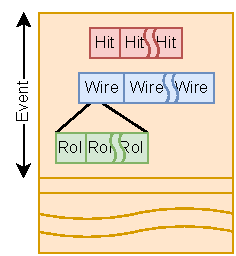
\includegraphics[width=\textwidth]{Figures/AOSLayout.pdf}
    \captionof{figure}{\scriptsize AOS Layout}

    \column{0.25\textwidth}
    \centering
    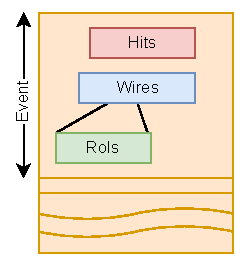
\includegraphics[width=\textwidth]{Figures/SOALayout.pdf}
    \captionof{figure}{\scriptsize SOA Layout}
  \end{columns}
\end{frame}

% -------- Granularity × Vertical‑split matrix --------
\begin{frame}{Granularity vs.\ Vertical Split Matrix}
\small\centering
\begin{tabular}{@{}lccc@{}}
\toprule
\textbf{\shortstack{Horizontal\\Granularity}} &
\textbf{\shortstack{1 NTuple\\(all DP)}} &
\textbf{\shortstack{1 NTuple\\/ DP}} &
\textbf{\shortstack{1 NTuple\\/ group}}\\
\midrule
Event‑wise      & \texttt{event\_allDP()}     & \texttt{event\_perDP()}     & \texttt{event\_perGroup()}\\
Spill‑wise      & \texttt{spill\_allDP()}     & \texttt{spill\_perDP()}     & \texttt{spill\_perGroup()}\\
Top‑object‑wise & --                                   & \texttt{topObject\_perDP()} & \texttt{topObject\_perGroup()}\\
Element‑wise    & --                                   & \texttt{element\_perDP()}   & \texttt{element\_perGroup()}\\
\bottomrule
\end{tabular}
\\[0.4em]
{\small DP = Data Product}
\end{frame}



\section{Parallel Optimizations}
\begin{frame}{Write Optimization: Multi-Threaded Chunking}
  % Vertically stacked code blocks for readability
  \textbf{Parallel Chunking}
  \small Divide events into thread-specific ranges for concurrent filling.
  \vspace{0.5em}
  \fbox{\parbox{0.95\textwidth}{\scriptsize
    \texttt{std::vector<unsigned int> seeds = generateSeeds(nThreads); }\\
    \texttt{for (int th = 0; th < nThreads; ++th) \{ }\\
    \hspace*{1.0em} \texttt{    int first = th * chunkSize; }\\
    \hspace*{1.0em} \texttt{    int last = std::min(first + chunkSize, totalEvents); }\\
    \hspace*{1.0em} \texttt{    futures.emplace\_back(std::async( }\\
    \hspace*{3.0em} \texttt{        std::launch::async, thinWorkFunc, first, last, seeds[th], th ));}\\
    \texttt{\} }
  }}
  \vspace{0.5em}
  \textbf{Example}: \texttt{executeInParallel} writers.

  \vspace{1em}


  \vspace{0.5em}
  \textbf{Project Use}: Scales writes with cores for large datasets.
\end{frame}

\begin{frame}{Read Optimization: Cluster-Aware Splitting}
  \textbf{Cluster Splitting}
  \small Split read ranges by cluster boundaries to avoid duplicates.
  \vspace{0.5em}
  \fbox{\parbox{0.95\textwidth}{\scriptsize
    \texttt{auto clusters = split\_range\_by\_clusters(*reader, nChunks); }\\
    \texttt{for (auto\& chunk : clusters) \{ }\\
    \hspace*{1.0em} \texttt{    futures.push\_back(std::async( }\\
    \hspace*{3.0em} \texttt{        \&processChunk, chunk.first, chunk.second }\\
    \hspace*{1.0em} \texttt{    )); }\\
    \texttt{\} }
  }}
  \vspace{0.5em}
  \textbf{Helper Function}
  \small Defines cluster-based splits.
  \vspace{0.5em}
  \fbox{\parbox{0.95\textwidth}{\scriptsize
    \texttt{std::vector<std::pair<size\_t, size\_t>> }\\
    \texttt{split\_range\_by\_clusters(ROOT::RNTupleReader\& reader, int nChunks) }
  }}
  \vspace{0.5em}
  \textbf{Project Use}: Enhances read efficiency by reducing redundant reads.
\end{frame}


% -------- Section: Challenges --------
\section{Challenges}
\begin{frame}{Challenge: Corrupted ROOT Files}
\centering
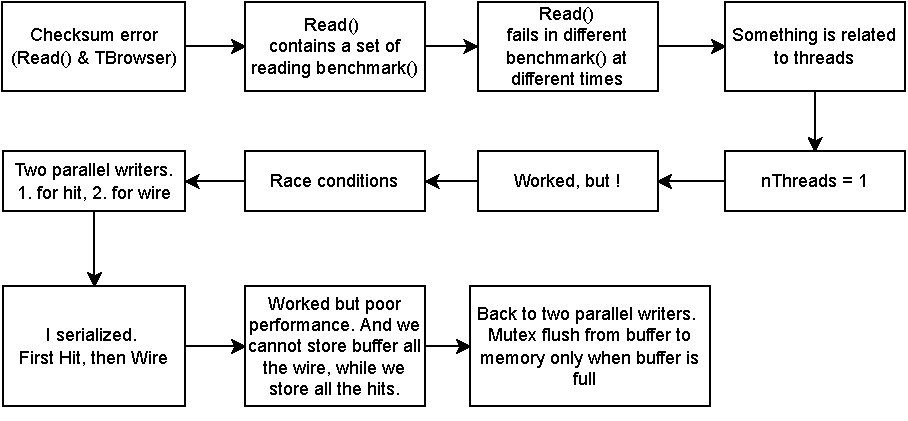
\includegraphics[width=0.9\linewidth]{Figures/Challenge.pdf}
\captionof{figure}{\scriptsize Challenge: Addressing corrupted ROOT files in parallel write operations.}
\end{frame}

\begin{frame}{Parallel Write Challenge: File Corruption Solution}
  \begin{columns}
    \column{0.4\textwidth}
    \textbf{Problem: Concurrent Flushes}
    \small Unsynchronized cluster flushes cause file corruption in multi-threaded writes.
    \vspace{0.5em}
    \textbf{Example Issue}: Threads overwriting shared file regions.

    \column{0.6\textwidth}
    \textbf{Solution: Mutex Synchronization}
    \small Lock during flushes to serialize access per cluster.
    \vspace{0.5em}
    \fbox{\parbox{0.9\textwidth}{\scriptsize
    \texttt{for (int idx = first; idx < last; ++idx) \{ }\\
    \hspace*{1.0em} \texttt{  // Generate data for hits/wires }\\
    \hspace*{1.0em} \texttt{  if (hitStatus.ShouldFlushCluster()) \{ }\\
    \hspace*{3.0em} \texttt{    hitContext.FlushColumns(); }\\
    \hspace*{3.0em} \texttt{    \{ }\\
    \hspace*{4.0em} \texttt{    std::lock\_guard<std::mutex> lock(mutex);  }\\
    \hspace*{3.0em} \texttt{    \} }\\
    \hspace*{3.0em} \texttt{    hitContext.FlushCluster(); }\\
    \hspace*{1.0em} \texttt{  \} }\\
    \texttt{\} }
    }}
    \vspace{0.5em}
    \textbf{Project Use}: Ensures thread-safe parallel writes without corruption.
  \end{columns}
\end{frame}
\begin{frame}{ROI Flattening vs. Custom Dictionary}
  \begin{columns}
    \column{0.5\textwidth}
    \textbf{ROI Flattening (Non-Dictionary)}
    \small Flattens hierarchical ROI data into vectors for efficient storage without custom classes.
    \vspace{0.5em}
    \fbox{\parbox{0.9\textwidth}{\scriptsize
    \texttt{struct Wires \{ }\\
    \hspace*{1.0em} \texttt{    vector<unsigned int> fSignalROI\_nROIs; }\\
    \hspace*{1.0em} \texttt{    vector<size\_t> fSignalROI\_offsets; }\\
    \hspace*{1.0em} \texttt{    vector<float> fSignalROI\_data; }\\
    \texttt{\}; }
    }}
    \vspace{0.5em}
    \textbf{Example}: Used in non-dictionary experiments for raw vector-based I/O.

    \column{0.5\textwidth}
    \textbf{Custom Dictionary (ROOT Classes)}
    \small Uses structured classes of ROOT's dictionary system, enabling object-oriented I/O.
    \vspace{0.5em}
    \fbox{\parbox{0.9\textwidth}{\scriptsize
    \texttt{struct RegionOfInterest \{ }\\
    \hspace*{1.0em} \texttt{    size\_t offset; }\\
    \hspace*{1.0em} \texttt{    vector<float> data; }\\
    \texttt{\}; }
    }}
    \vspace{0.5em}
    \textbf{Example}: Used in dictionary experiments for type-safe, hierarchical data handling.
  \end{columns}
  \vspace{1em}
\end{frame}


% -------- Section: Results --------
\section{Results}

\begin{frame}{Evaluation Metrics}
\small
\begin{itemize}
  \item \textbf{Write Throughput:} Total events per second during RNTuple serialization.
  \item \textbf{Cold Read Time:} Latency for first access after file creation, reflecting raw I/O.
  \item \textbf{Warm Read Time:} Latency when data is cached, measuring memory locality effects.
  \item \textbf{Compressed File Size:} Total on-disk footprint post-write, accounting for RNTuple's column-wise compression.
\end{itemize}
\end{frame}

% Experimental setup (added after Evaluation Metrics)
\begin{frame}{Experimental Setup}
\footnotesize
\begin{columns}[t,onlytextwidth]
  \column{0.58\textwidth}
  \textbf{Hardware}\\
  \vspace{1em}
  \begin{tabular}{@{}l p{0.68\linewidth}@{}}
  CPU & Intel Xeon Silver 4214R @ 2.40\,GHz \\
  Cores/Threads & 12 cores per socket, 24 threads (HT) \\
  Memory & 94\,GB RAM \\
  Storage & SSD: 540\,MB/s read, 520\,MB/s write \\
  \end{tabular}

  \column{0.40\textwidth}
  \textbf{Benchmark Parameters}\\
  \vspace{1em}
  \begin{tabular}{@{}l r@{}}
  Events & 1\,M \\
  Hits per event & 100 \\
  Wires per event & 100 \\
  ROIs per wire & 10 \\
  Spills & 10 \\
  \end{tabular}
\end{columns}
\end{frame}

\begin{frame}{AOS: Write Performance}
  \centering
  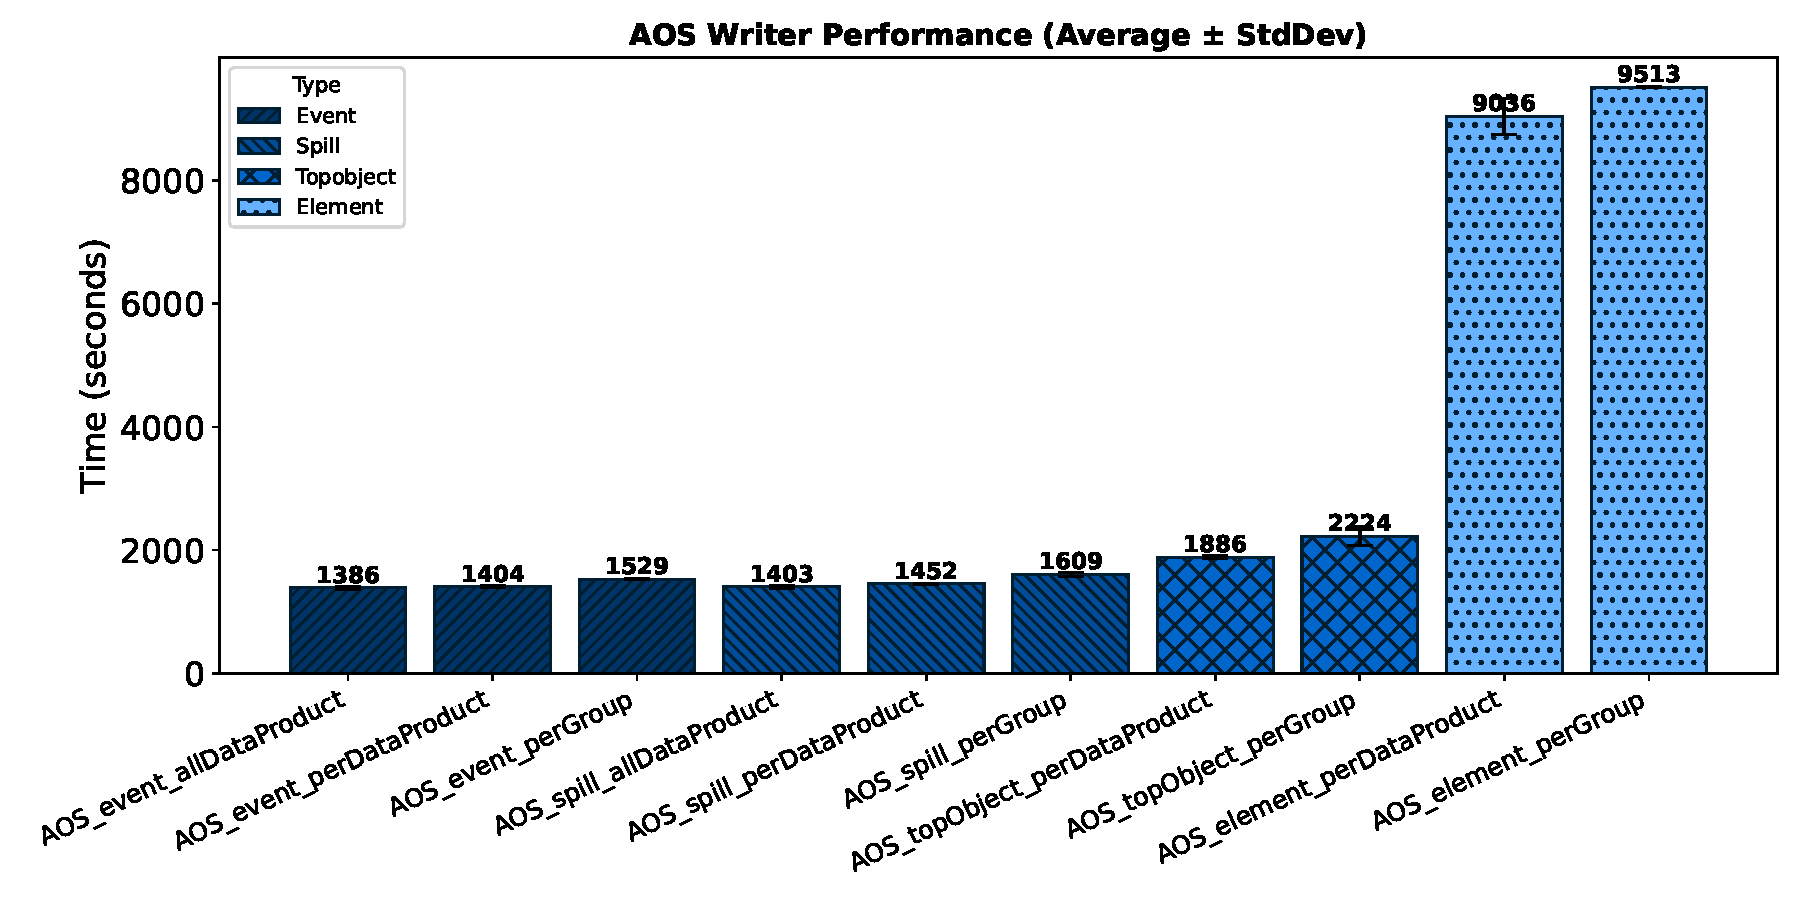
\includegraphics[width=0.9\linewidth]{../experiments/Seaborn/AOSWriter_blue_shaded.pdf}
  \captionof{figure}{\scriptsize AOS (Array of Structures) Write performance across different persistent layouts.}
\end{frame}

\begin{frame}{AOS: Write Performance}
\centering
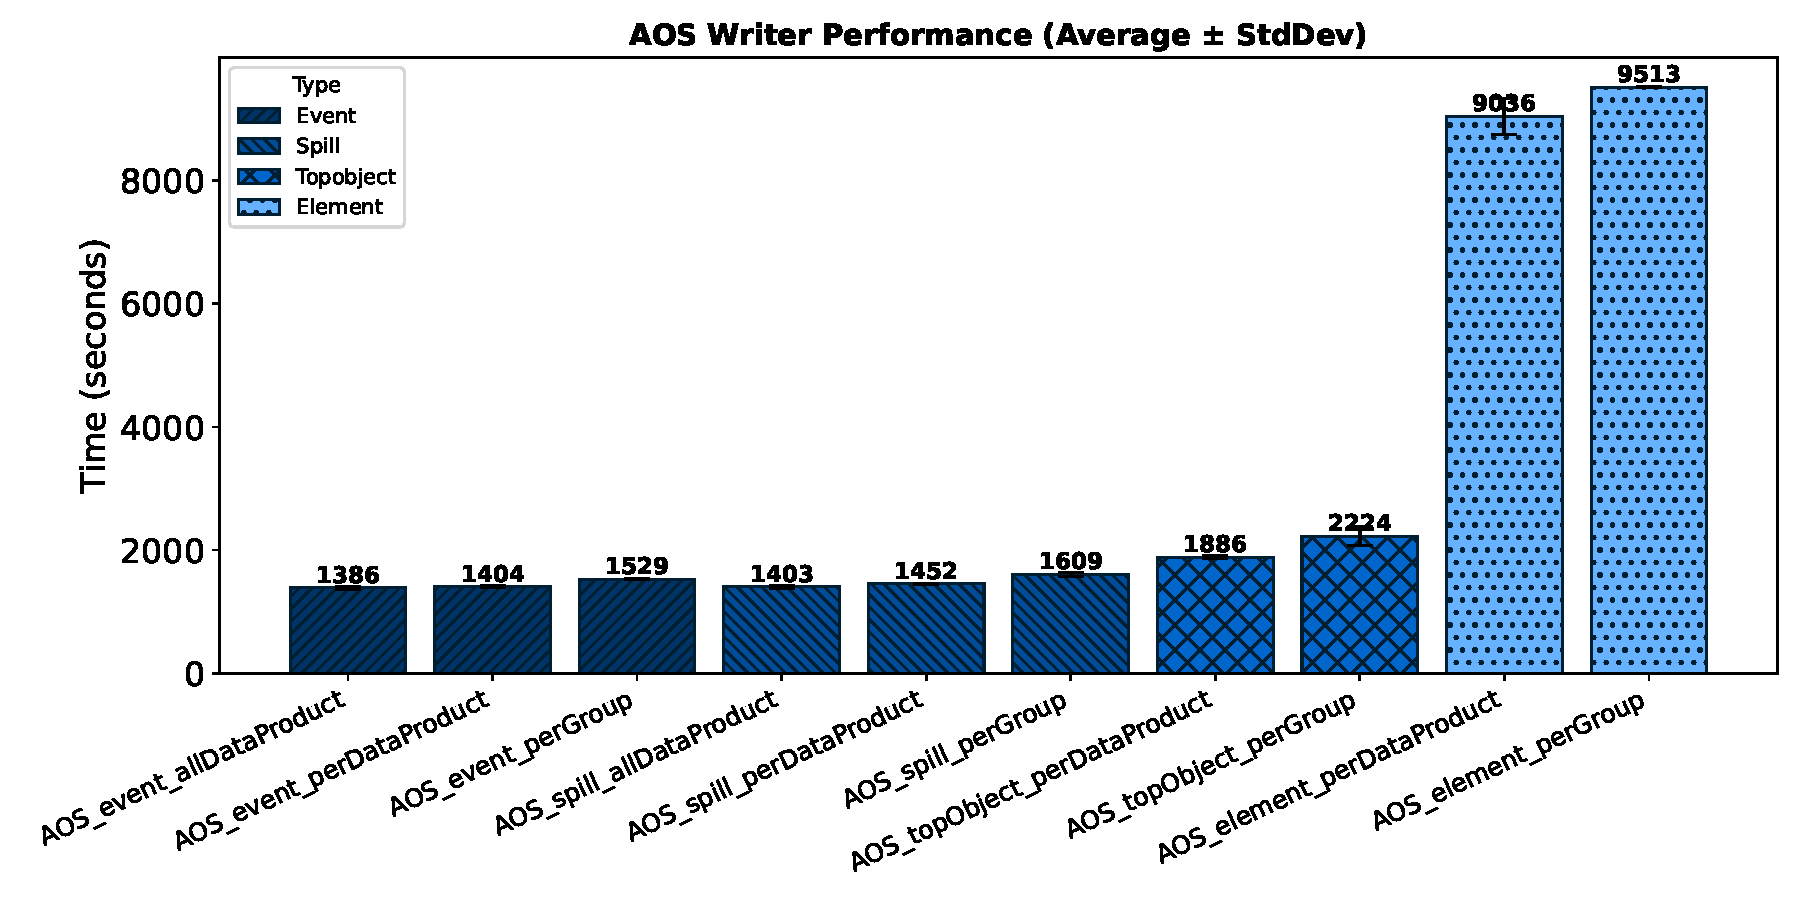
\includegraphics[width=0.5\linewidth]{../experiments/Seaborn/AOSWriter_blue_shaded.pdf}

\textbf{Key Takeaways:}
\begin{itemize}
\item Higher granularity leads to slower write performance, mainly due to thread contention.
\item For horizontal persistent layouts, slow down is upto $6.9\times$, although it is marginal for vertical persistent layouts.
\end{itemize}
\end{frame}

\begin{frame}{SOA: Write Performance}
\centering
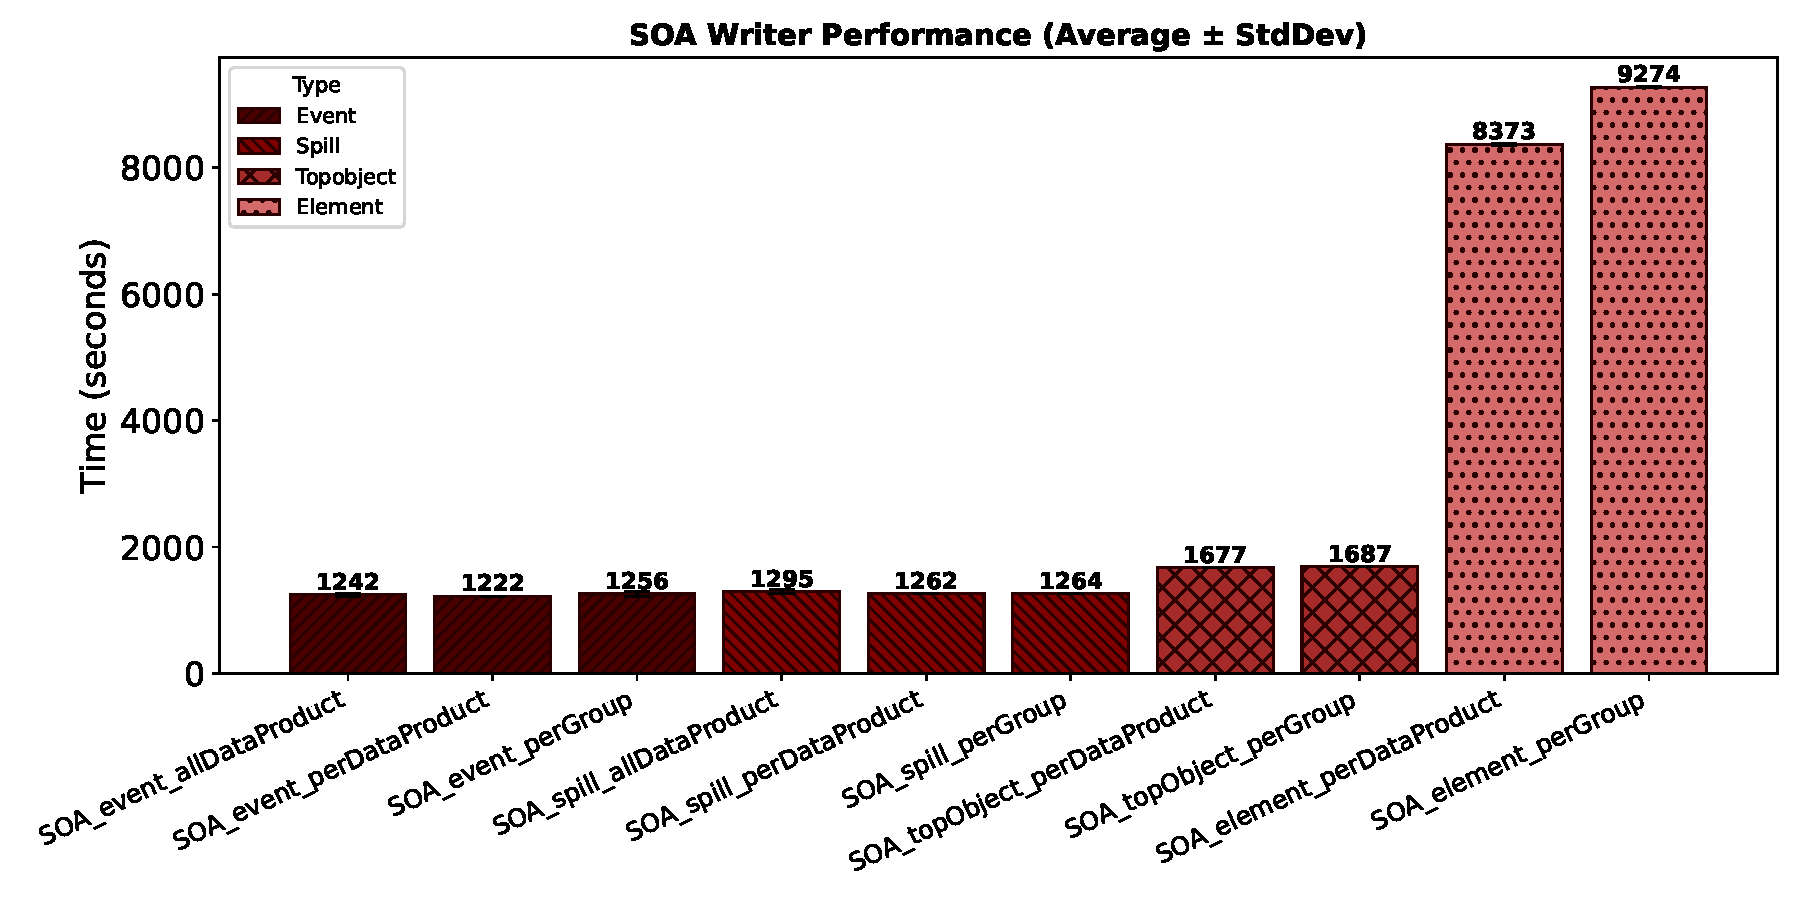
\includegraphics[width=0.9\linewidth]{../experiments/Seaborn/SOAWriter_shaded.pdf}
\captionof{figure}{\scriptsize SOA (Structure of Arrays) Write performance across different persistent layouts.}
\end{frame}

\begin{frame}{SOA: Write Performance}
  \centering
  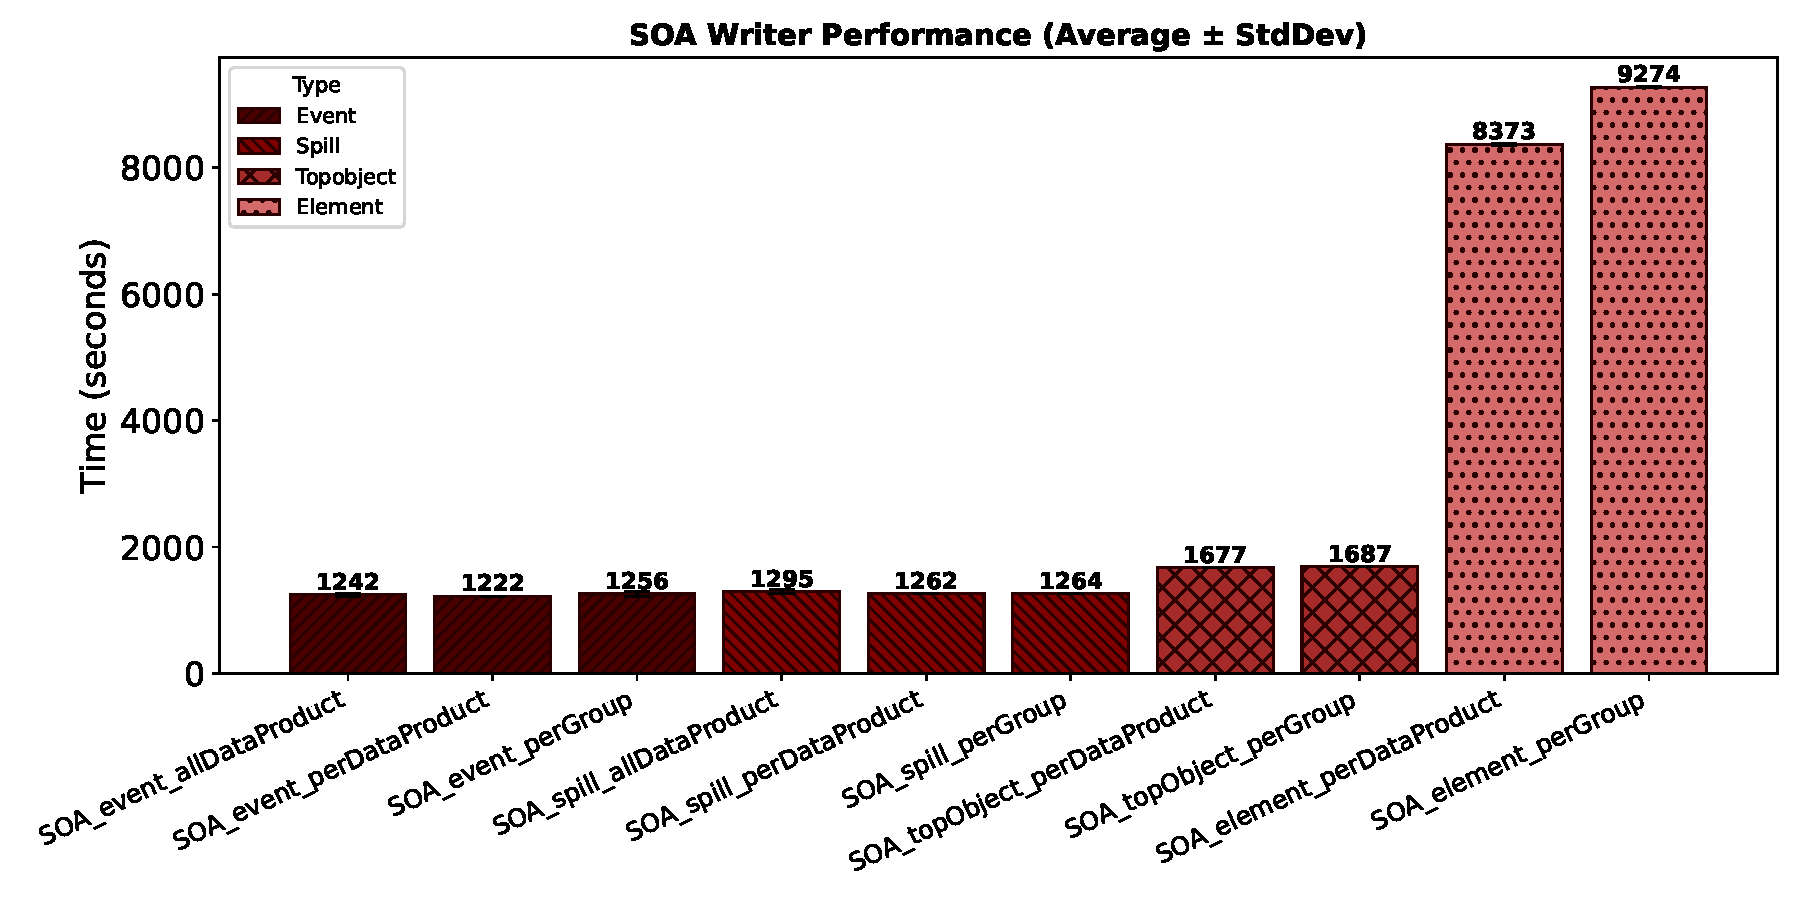
\includegraphics[width=0.5\linewidth]{../experiments/Seaborn/SOAWriter_shaded.pdf}
  
  \textbf{Key Takeaway:}
  \begin{itemize}
  \item SOA writer performance is overall similar to AOS writer performance.

  \end{itemize}
\end{frame}


\begin{frame}{AOS vs SOA: Write Performance}
  \centering
  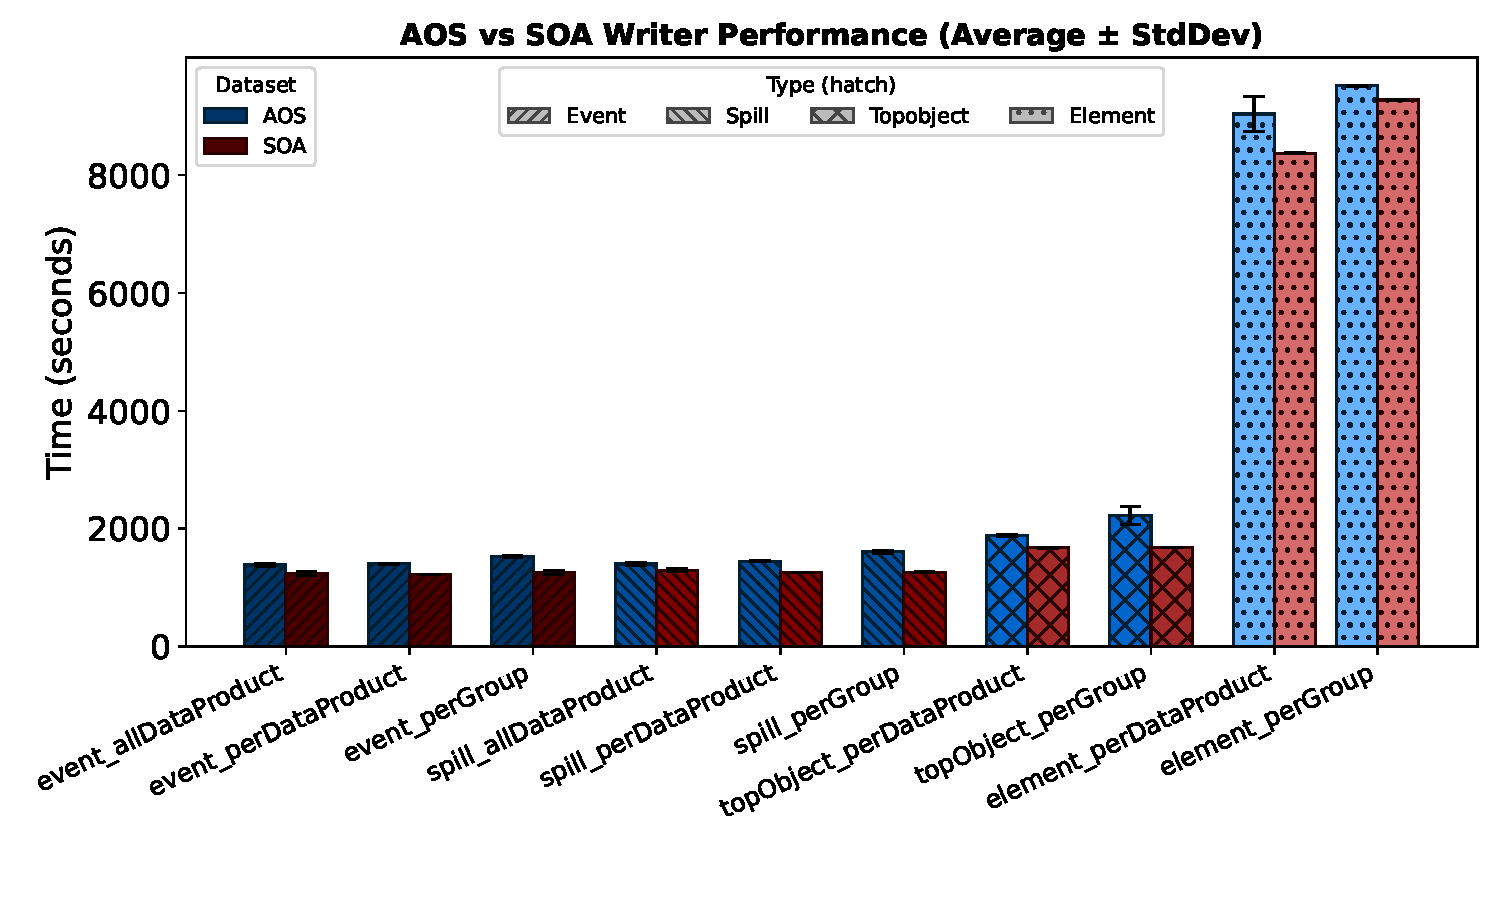
\includegraphics[width=0.8\linewidth]{../experiments/Seaborn/AOS_SOA_Writer_grouped_with_gaps.pdf}
  \captionof{figure}{\scriptsize AOS vs SOA write performance across different persistent layouts.}
\end{frame}

\begin{frame}{AOS vs SOA: Write Performance}
  \centering
  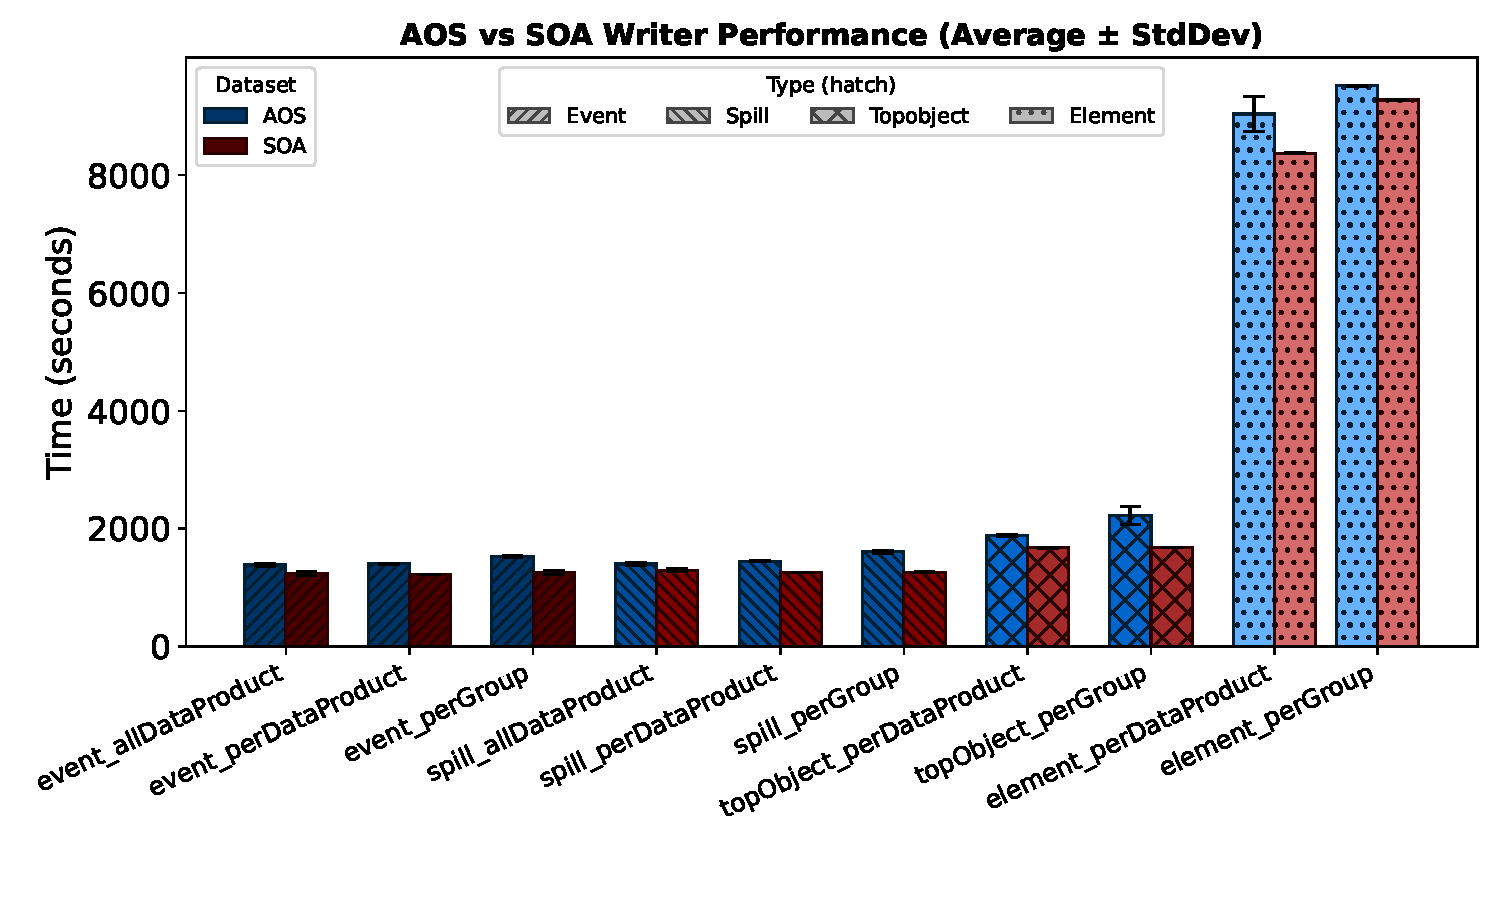
\includegraphics[width=0.5\linewidth]{../experiments/Seaborn/AOS_SOA_Writer_grouped_with_gaps.pdf}

  \textbf{Key Takeaway:}
  \begin{itemize}
  \item SOA writer is on average $3.65\%$ faster than AOS writer for all persistent layouts.

  \end{itemize}
\end{frame}

% \begin{frame}[c]{CPU Time Overheads}
%   \small
%   \begin{columns}[c,onlytextwidth]
%     \column{0.55\textwidth}
%     \footnotesize
%     \begin{tabular}{lccc}
%       \toprule
%       Writer & A & B & C\\
%       \midrule
%       \texttt{event\_perGroup}   & \checkmark & \checkmark & \\
%       \texttt{spill\_perGroup}   & \checkmark & \checkmark & \checkmark\\
%       \texttt{element\_perData}  & \checkmark & \checkmark & \\
%       \texttt{topObject\_perData}&   & \checkmark & \\
%       \texttt{event\_perData}    &   & \checkmark & \\
%       \texttt{spill\_perData}    &   & \checkmark & \checkmark\\
%       \bottomrule
%     \end{tabular}
%     \column{0.45\textwidth}\\[0.3em]
%     \begin{itemize}
%       \item \textbf{A – ROI flattening:} dominant for *element* and *perGroup* writers.
%       \item \textbf{B – Multiple NTuples:} extra \texttt{Fill}/Flush cycles \& mutex contention.
%       \item \textbf{C – Spill re-partitioning:} additional work unique to *spill* writers.
%     \end{itemize}
%   \end{columns}
%   \end{frame}

\begin{frame}{File Size Analysis: AOS vs SOA}
  \begin{columns}[T,onlytextwidth]
    \column{0.5\textwidth}
    \centering
    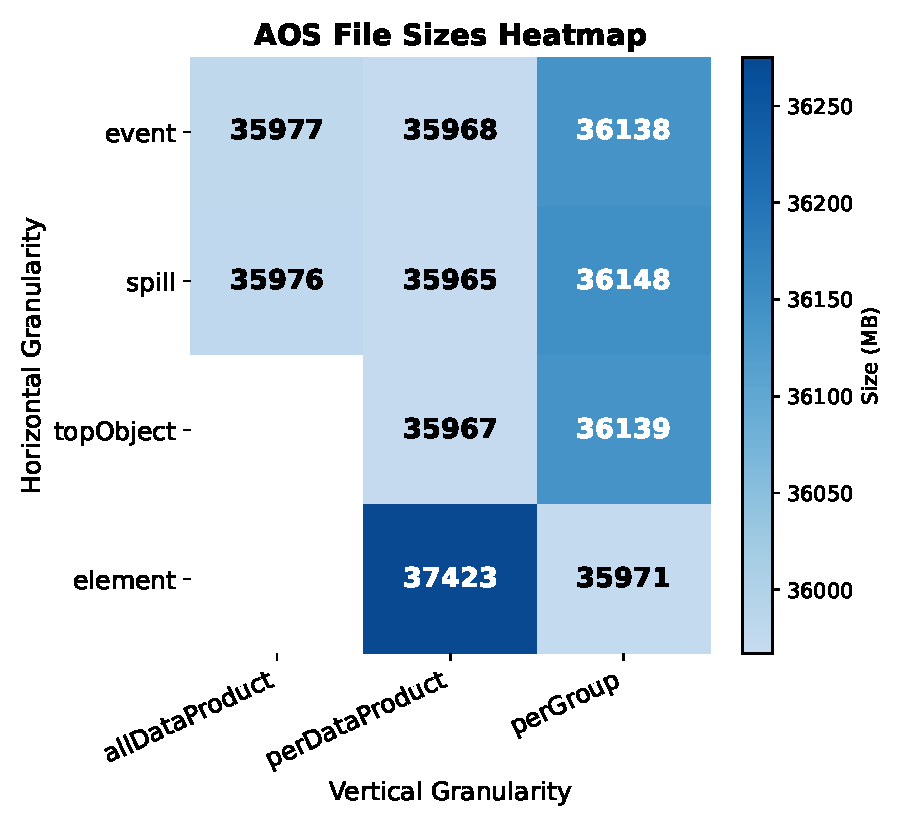
\includegraphics[width=\linewidth]{../experiments/Seaborn/AOS_FileSize_Heatmap_softblue_nogrid.pdf}
    \captionof{figure}{\scriptsize AOS file size across persistent layouts}

    \column{0.5\textwidth}
    \centering
    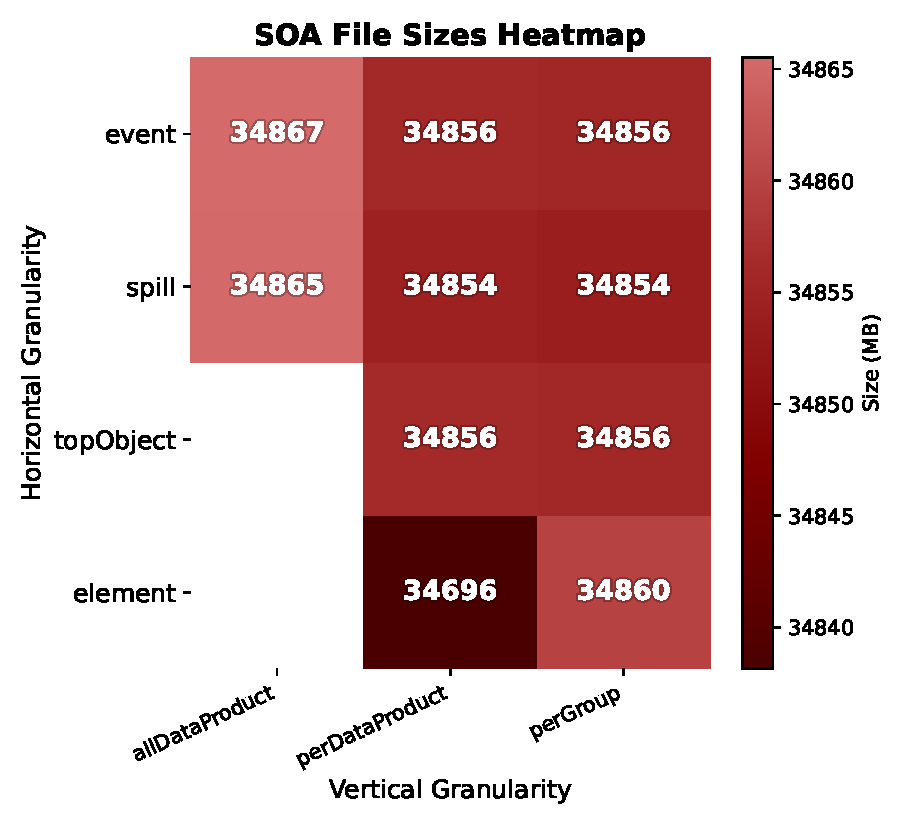
\includegraphics[width=\linewidth]{../experiments/Seaborn/SOA_FileSize_Heatmap_merun_white.pdf}
    \captionof{figure}{\scriptsize SOA file size across persistent layouts}
  \end{columns}
\end{frame}

\begin{frame}{File Size Analysis: AOS vs SOA}
  \centering
  \makebox[\textwidth]{
    \begin{minipage}[t]{0.38\textwidth}
      \centering
      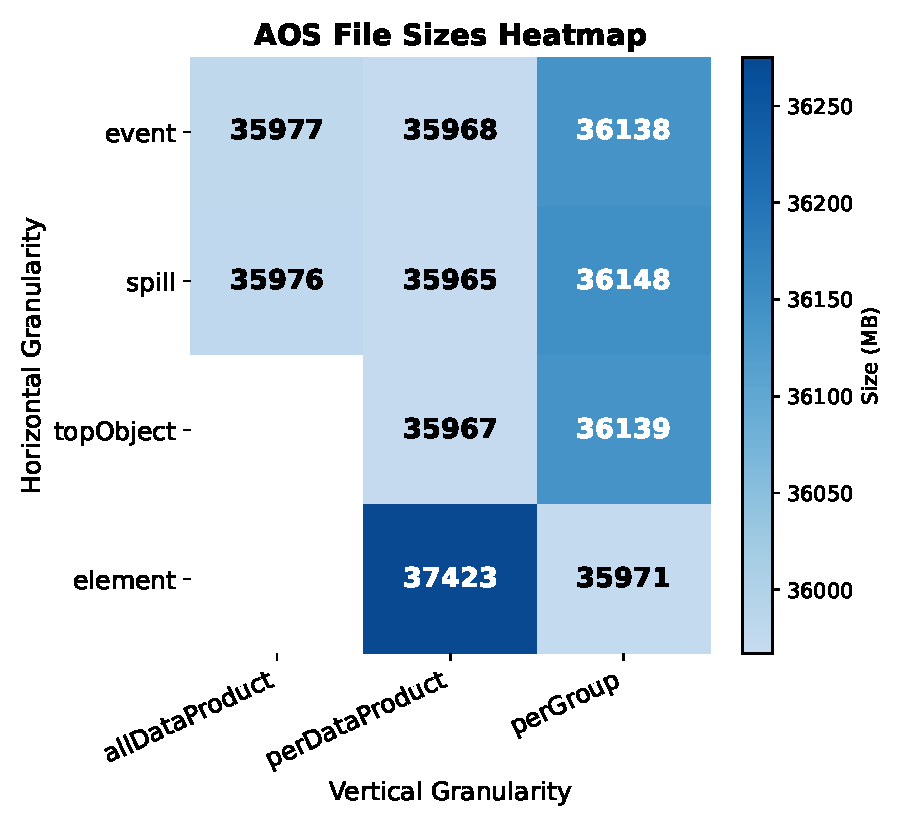
\includegraphics[width=\linewidth]{../experiments/Seaborn/AOS_FileSize_Heatmap_softblue_nogrid.pdf}
    \end{minipage}
    \hspace{0.04\textwidth}
    \begin{minipage}[t]{0.38\textwidth}
      \centering
      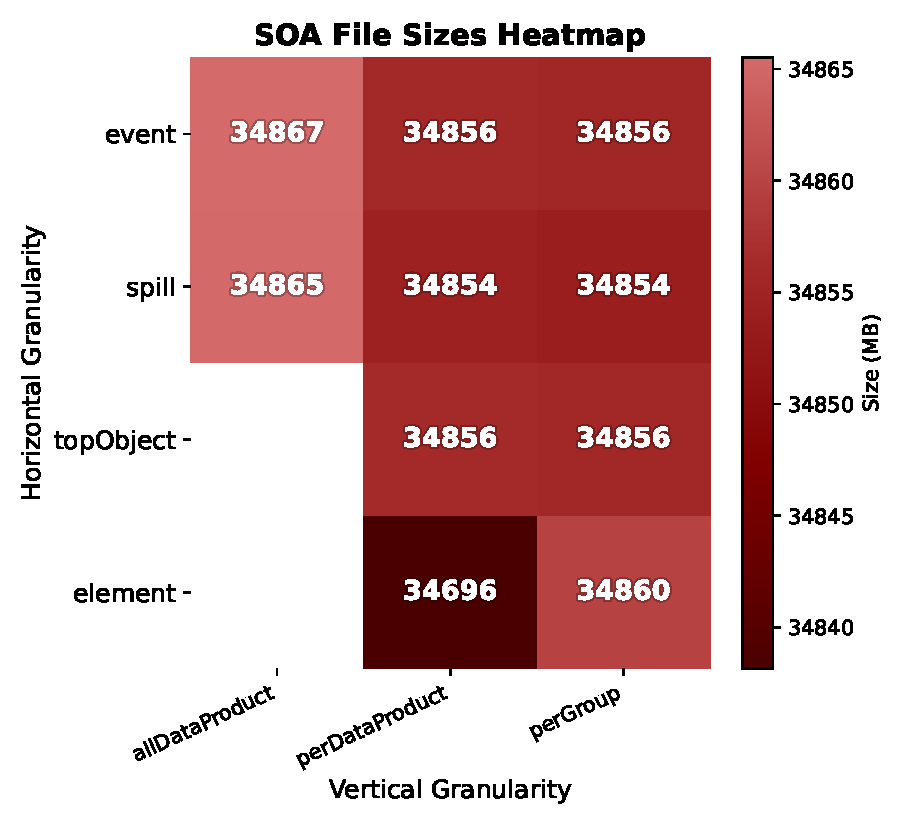
\includegraphics[width=\linewidth]{../experiments/Seaborn/SOA_FileSize_Heatmap_merun_white.pdf}
    \end{minipage}
  }
  \textbf{Inconclusive observations:}
  \begin{itemize}
    \item The variability in file size is higher for AOS than SOA.
    \item Element\_perDataProduct layout for AOS leads to higher file size due to additional information storage of EventID and WireID. 
  \end{itemize}
\end{frame}

\begin{frame}{Fields Read in Benchmarks}
\small
\begin{itemize}
  \item \textbf{Hits}: \texttt{PeakAmplitude}.
  \item \textbf{Wires}: \texttt{Channel}.
  \item \textbf{ROIs}: ROI data vector \texttt{data}.
  \vspace{1.5em}
  \item \textbf{Note}: We do not reconstruct full objects from the fields; we only read the fields through RNTuple views, using \texttt{volatile} to prevent the compiler optimization.
\end{itemize}
\end{frame}

\begin{frame}{AOS vs SOA: Cold Read Performance Comparison}
\centering
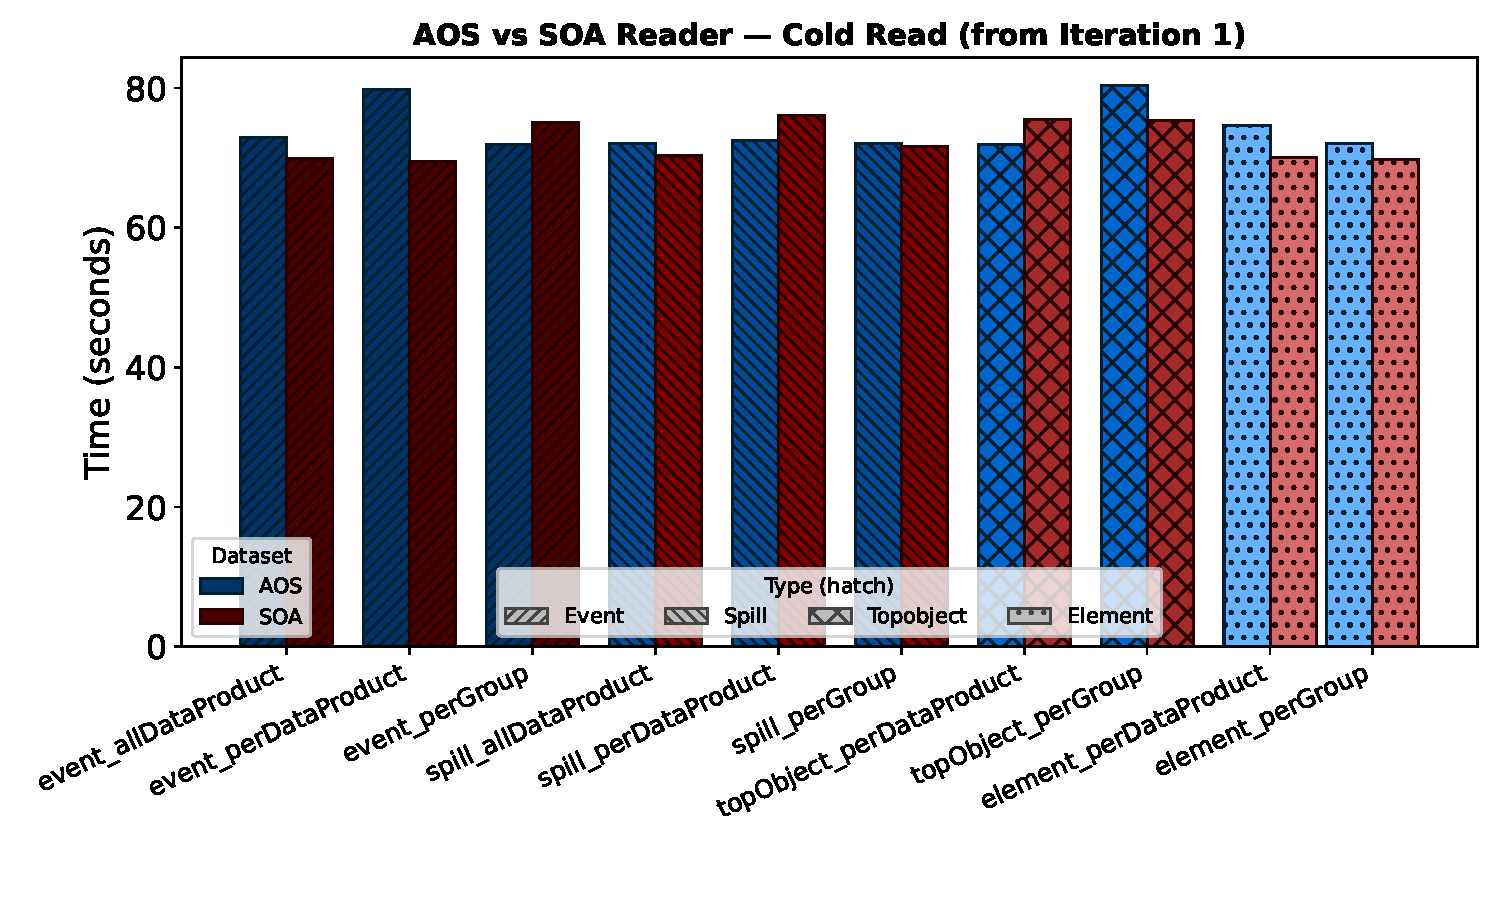
\includegraphics[width=0.8\linewidth]{../experiments/Seaborn/AOS_SOA_Reader_Cold_grouped_progressive.pdf}
\captionof{figure}{\scriptsize Cold Read Performance Comparison: Initial read times for AOS vs SOA implementations.}
\end{frame}

\begin{frame}{AOS vs SOA: Cold Read Performance Comparison}
  \centering
  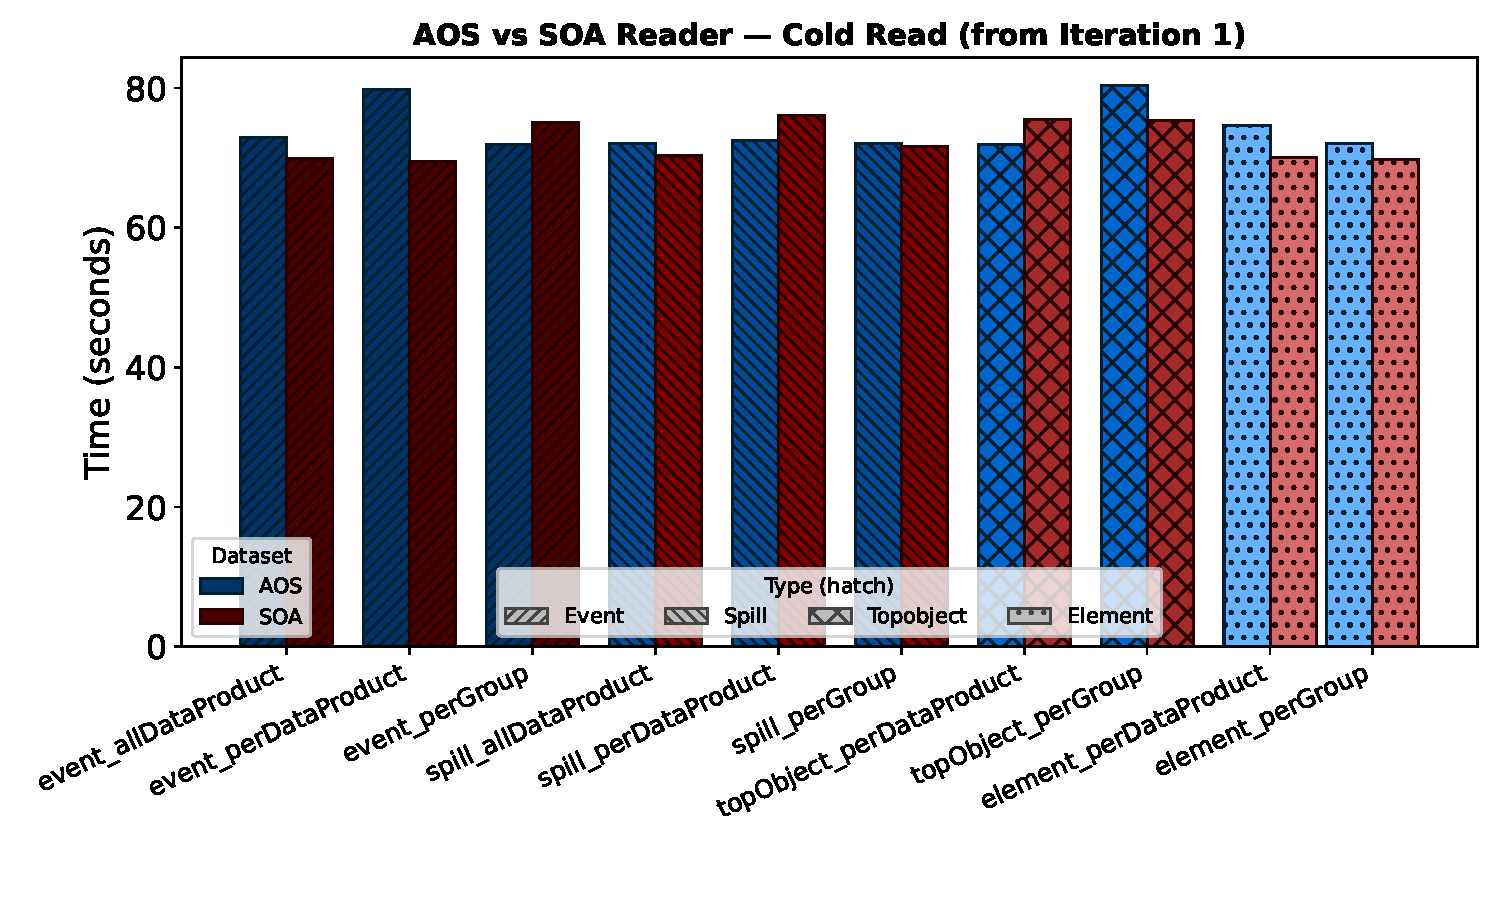
\includegraphics[width=0.6\linewidth]{../experiments/Seaborn/AOS_SOA_Reader_Cold_grouped_progressive.pdf}
  
  \textbf{Inconclusive observations:}
  \begin{itemize}
  \item SOA reader is on average $2.34\%$ faster than AOS reader for cold read.
  \end{itemize}
  \end{frame}

\begin{frame}{AOS vs SOA: Warm Read Performance Comparison}
\centering
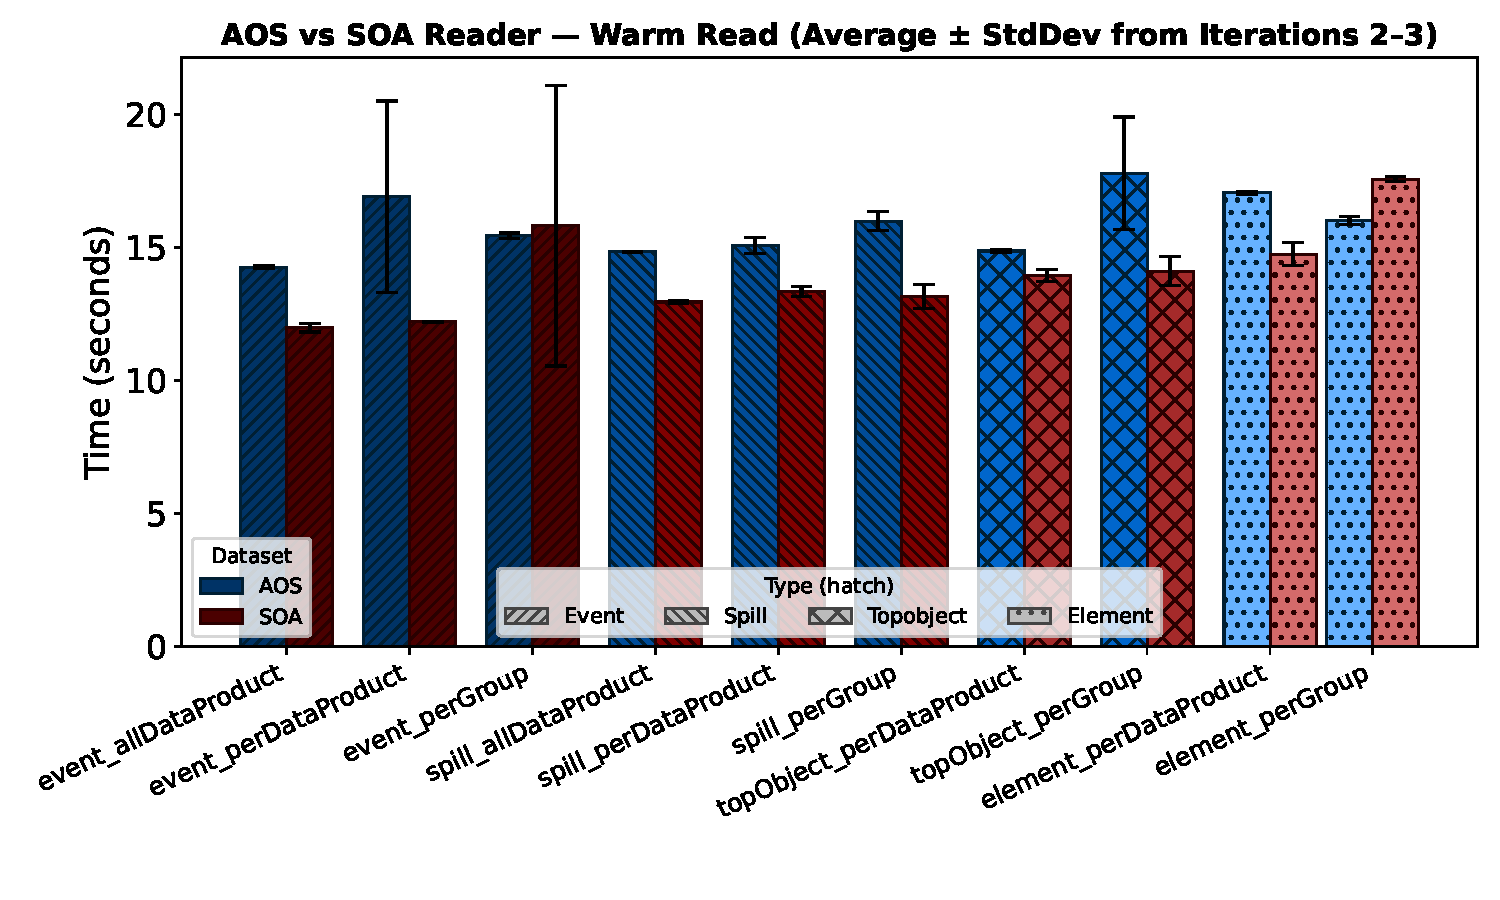
\includegraphics[width=0.8\linewidth]{../experiments/Seaborn/AOS_SOA_Reader_Warm_grouped_progressive.pdf}
\captionof{figure}{\scriptsize Warm Read Performance Comparison: Subsequent read times for AOS vs SOA implementations.}
\end{frame}

\begin{frame}{AOS vs SOA: Warm Read Performance Comparison}
  \centering
  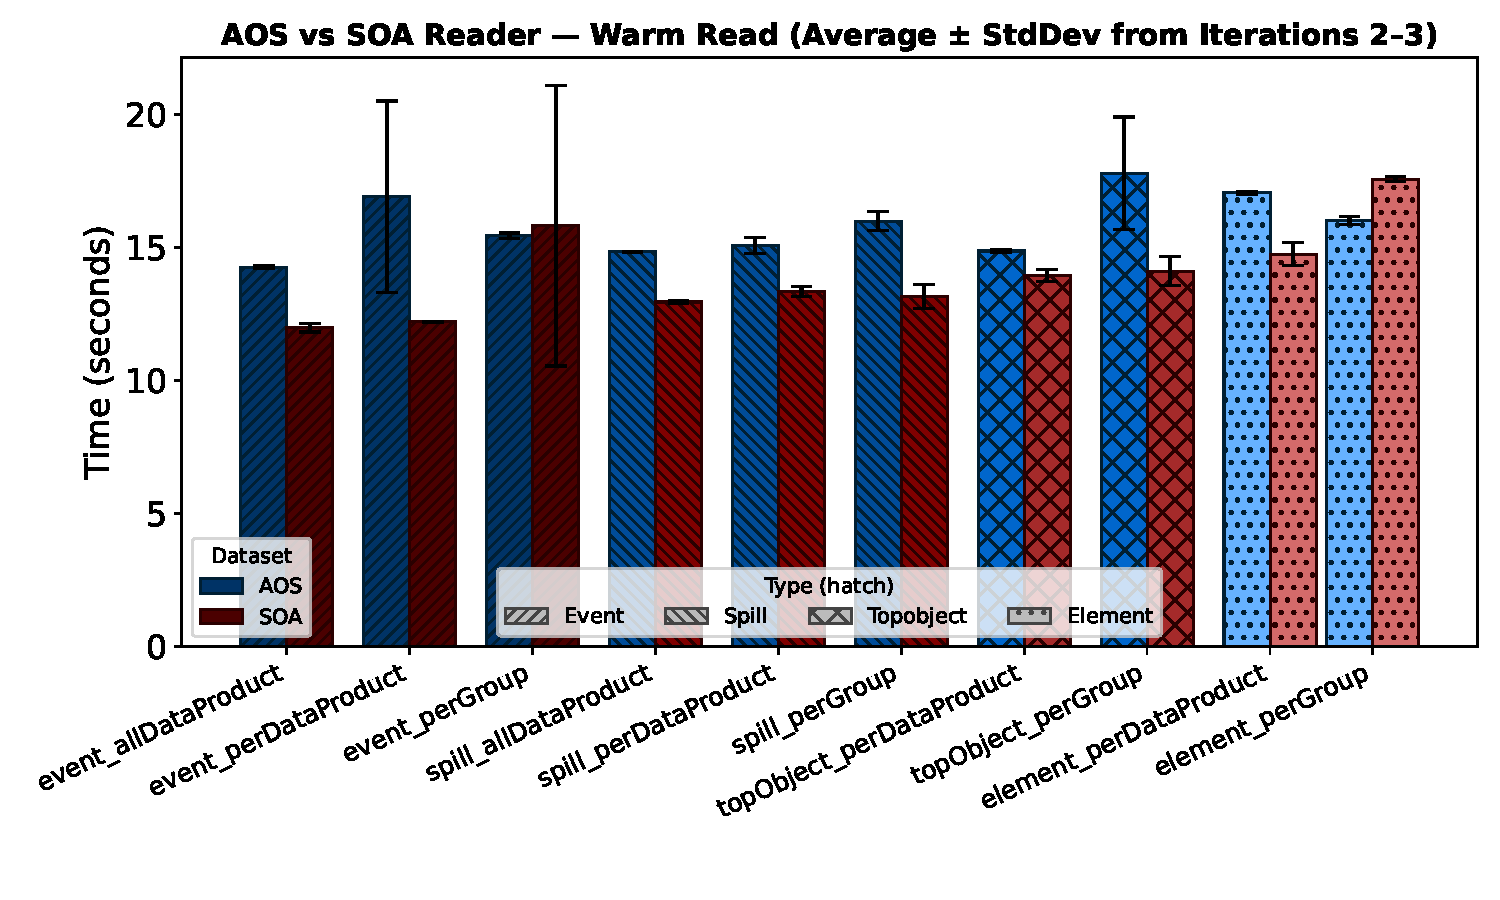
\includegraphics[width=0.6\linewidth]{../experiments/Seaborn/AOS_SOA_Reader_Warm_grouped_progressive.pdf}
  
  \textbf{Inconclusive observations:}
  \begin{itemize}
  \item Average warm read is $4.91\times$ faster than cold read across all persistent layouts.
  \item SOA reader is on average $11.63\%$ faster than AOS reader for warm read.
  \end{itemize}
  \end{frame}


\begin{frame}{Future Considerations}
\begin{itemize}

  \item \textbf{Uniformity in Data Storage:} Deterministic approach to store exactly same data for each of the root files.

  \vspace{0.5em}

  \item \textbf{Thread Scaling Analysis:} Rigorous testing across 1--128 threads to evaluate layout performance scaling and optimal configurations.
  
  \vspace{0.5em}
  
  \item \textbf{Extensible Framework:} Develop scalable architecture for arbitrary data products beyond Hits and Wires with configurable layouts.
  
  \vspace{0.5em}
  
  \item \textbf{Advanced Layout Testing:} Explore N-tuple groupings and clustering strategies for improved read/write efficiency and storage optimization.
\end{itemize}
\end{frame}

% References Slide
\begin{frame}{References}
\small
[1] DUNE Collaboration, “Deep Underground Neutrino Experiment Technical Design Report– VolumeII: DUNE Physics,” 2020, Sec.2.6.\par
[2] DUNE Collaboration, “Data Acquisition System for the DUNE Far Detector,” IEEE NSS/MIC Proc., 2023.\\
\end{frame}

% Final Slide
\begin{frame}[standout]
\large Source code: \url{https://github.com/Framework-R-D/phlex-io-granularity-test}
\vspace{3em}\\
Thank you! \\
Questions?\\[0.8em]
\end{frame}

\end{document}
